\chapter[Lecture 22]{}\label{lec22}

Two independent orientation for different spines make total no. of orbitals (distinct) $=2N$.

If each atom contribute 1 electron in the band, the band will be half filled.

If each atom contributes two electrons, the band will be completely filled.
\begin{figure}[H]
\centering
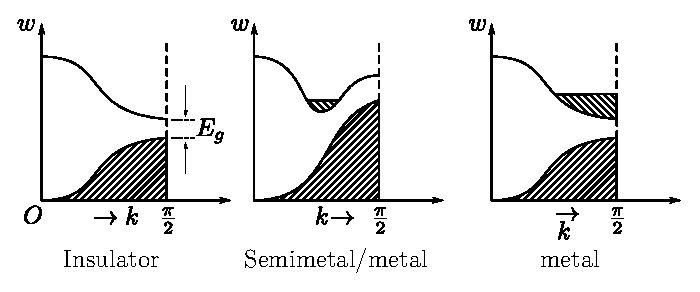
\includegraphics{images/lecture22/fig1.eps}
\end{figure}
Direct gap $\to$ Energy difference between top of valence band and bottom of conduction band at same $k$.

Indirect gap $\to$ If the above is not true.
\begin{figure}[H]
\centering
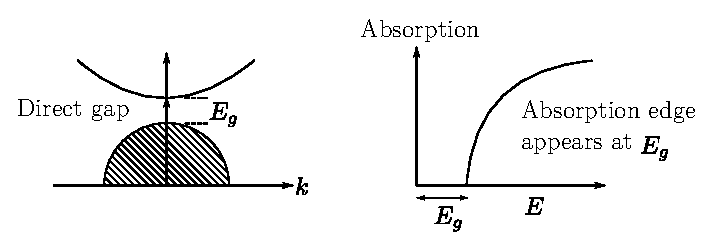
\includegraphics{images/lecture22/fig2.eps}
\end{figure}
A phonon of wave vector $k$ and frequency $\Omega$ is created in the absorption process.
$$
\therefore\quad \hbar w=E_{g}+\hbar \Omega
$$
\begin{figure}[H]
\centering
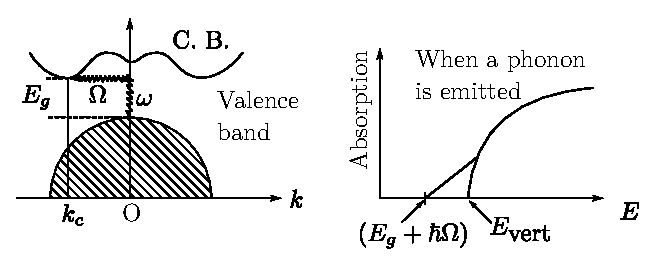
\includegraphics{images/lecture22/fig3.eps}
\end{figure}
Energy and momentum are conserved for electronic transitions. Therefore, the transitions across $E_{g}$ is difficult for indirect gap.

Absorption threshold for the indirect transition between the band edge is at $\hbar w=E_{g}+\hbar\Omega$, $\Omega$ is the frequency of emitted phonon of wave vector $K\simeq -k_{C}$ = phonon momentum $K(\text{photon})=k_{C}+K\simeq 0$ at low energies $\Rightarrow K=-K_{C}$. At high temp, phonon and are occupied $\to$ if a phonon is absorbed along with the photon, threshold energy $=E_{g}-\hbar\Omega=\hbar w$.

Indirect gap $\to$ phonons are required for excitations.

$\to$ Band gap can be found from temperature dependence of absorption edge.

Although $\sim$ is linear in $k$ at band minimum, it reaches maxima at inflection  point of the band and then becomes smaller, as if there is acceleration of the electrons opposite to the applied external electric force. This extra ordinary scenario is a consequence of periodic potential, which although no longer explicit in semi classical theory lies buried in it. As electron approaches a Bragg plane, the external field move it towards levels in which it is likely to get Bragg reflected.




